\section{我不知道}

六經之道同歸,而禮樂之用為急,治身者斯須忘禮,則暴嫚入之矣。為國者一朝失禮,則荒亂及之矣。人函天地陰陽之氣,有喜怒哀樂之情,天禀其性,而不能節也。聖人能為之節而不能絕也。故象天地而制禮樂,所以通神明,立人倫,正情性,節萬事者也。

RLC回路は、抵抗 (resistor)、コイル (inductor)、コンデンサ (capacitor) を直列または並列に接続した回路のことです。

The quick brown fox jumps over the lazy dog.

微分方程式とは、ある関数とその導関数を含む方程式のことです。
例えば、\(x\) の関数 \(y\) とその導関数 \(\dv{y}{x}\)を含んだ式は微分方程式といえます。
この方程式を満たす「関数 \(y\)」がこの方程式の解であり、これを求めることを「\emph{微分方程式を解く}」といいます。

\begin{figure}[htb]
	\centering
	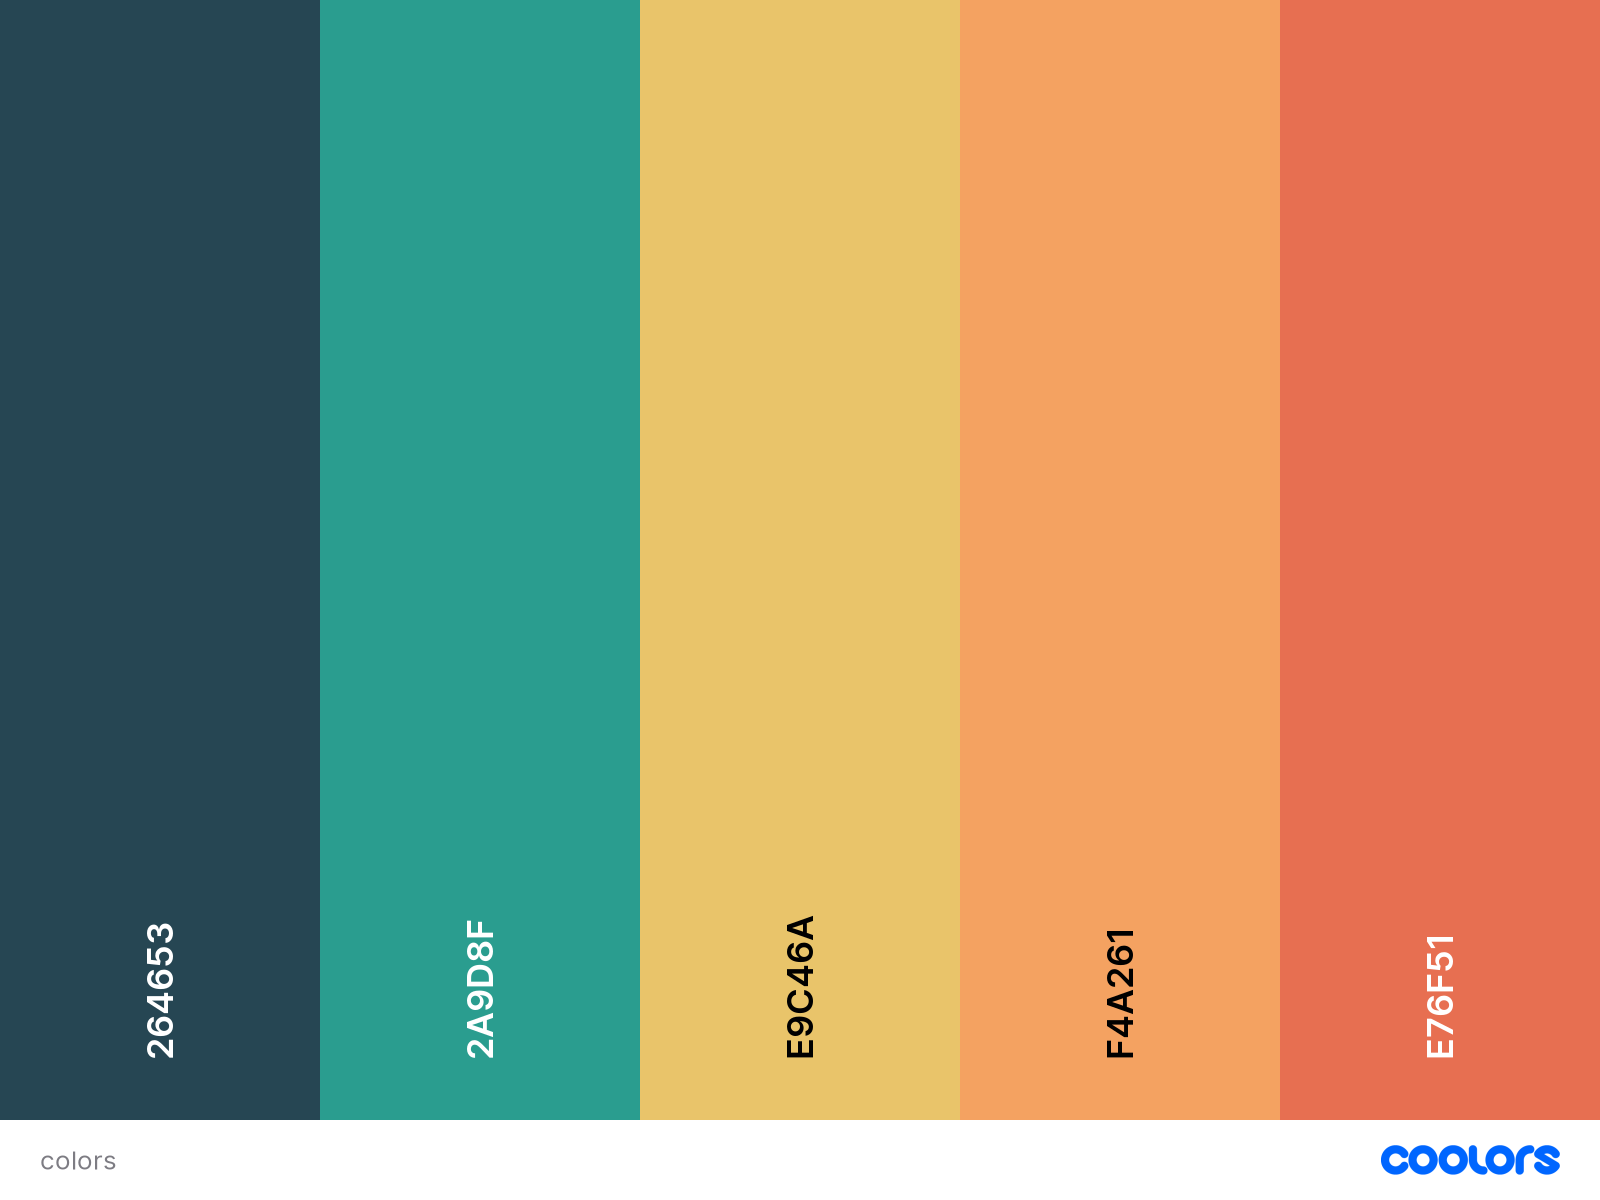
\includegraphics[width=0.5\textwidth]{colors.png}
	\caption{色々な色}
	\label{fig:colors}
\end{figure}

citation \cite{sizesuu}
